\chapter{Theoretical Framework I: Single-Aperture Optics}
\label{ch:single}

\section{The reduced eye model}
\label{sec:reduced-eye}
Every optical calculation in this project uses the standard \emph{reduced eye}
simplification: the cornea, aqueous, crystalline lens, and vitreous are lumped into a
single refracting surface of power $P_0$, situated at one plane, imaging directly onto
the retina. This is the same simplification underlying the Gullstrand--Emsley reduced
eye and is what makes a single scalar $P_0$ meaningful at all; it deliberately does not
model the cornea/lens power split (roughly 2:1 in a real eye), nor the physical
anterior-chamber depth ($\approx 3.6$\,mm) separating them. This choice is stated
explicitly in \texttt{stage2\_fixed/phase2\_retina.py}'s own module docstring
(PHYSICS\_AUDIT.md item E1, verified present in that file, mtime -- see
Chapter~\ref{ch:provenance}) precisely so a reader cannot mistake it for an oversight.

The values used throughout are:
\begin{center}
\begin{tabular}{lll}
\toprule
Symbol & Value & Meaning \\
\midrule
$P_0$ & $60.0$\,D & Total (emmetropic) reduced-eye power \\
$n'$ & $1.336$ & Refractive index of the vitreous humour \\
$D_{\mathrm{pupil}}$ & $4000\,\mu$m & Photopic pupil diameter \\
$\lambda$ & $550$\,nm & Vacuum design wavelength (photopic luminous peak) \\
$d_{\mathrm{gap}}$ & $12$\,mm & Spectacle-plane vertex distance, pinhole to cornea \\
\bottomrule
\end{tabular}
\end{center}
(source: \texttt{stage2\_fixed/myopia\_axial.py}, \texttt{new\_sweeps/run\_acuity\_sweep.py}
constants \texttt{WAVELENGTH\_NM=550.0}, \texttt{D\_GAP\_MM=12.0}; see
Chapter~\ref{ch:provenance} for exact mtimes).

\subsection{Axial myopia model}
This project models myopia as \emph{axial}, not \emph{refractive}: the eye's total power
$P_0$ is held fixed at its emmetropic value for every degree of myopia $M$; only the
eye's axial length grows, pushing the retina past the eye's own (unchanged) focal point.
This is the defining choice of \texttt{stage2\_fixed/myopia\_axial.py}
(\texttt{axial\_length\_for\_myopia}, verified read directly):
\begin{align}
L_0 &= \frac{n'}{P_0} & \text{(emmetropic axial length, fixed reference)}\\
L_{\mathrm{ax}}(M) &= \frac{n'}{P_0-M} & \text{(myopic axial length for this } M \text{)}\\
f_{\mathrm{eye}} &= L_0 & \text{(eye power fixed at the emmetropic value for every } M\text{)}
\end{align}
The alternative -- a \emph{refractive} model, in which $P_0$ itself changes with $M$
while axial length stays fixed -- was not implemented; the axial convention was chosen
because it is the anatomically dominant mechanism in real myopia (axial elongation of
the globe) and because it lets one physical eye power $P_0$ be reused unmodified across
the entire $M$ sweep. With $P_0=60$D and $n'=1.336$: $f'_{\mathrm{image}} =
n'/P_0\times10^6 = 22{,}266.667\,\mu$m -- the media-reduced image distance, not the naive
vacuum value $1/P_0$.

\section{Geometric blur, diffraction blur, and the stenopeic effect}
\label{sec:stenopeic}
An uncorrected myopic eye focuses light from a distant object \emph{in front of} the
retina; by the time the diverging cone reaches the actual retinal plane it has spread
into a geometric blur circle of radius approximately proportional to the eye's pupil
diameter and to the degree of defocus. A pinhole of diameter $a_{\mathrm{hole}} \ll
D_{\mathrm{pupil}}$ placed in front of the eye restricts the admitted ray bundle to a
much narrower cone, shrinking that geometric blur circle in direct proportion to
$a_{\mathrm{hole}}$ -- the stenopeic (``narrow-aperture'') effect, and the entire
physical basis for treating a small aperture as a myopia correction at all.

This benefit is not free. Diffraction at the aperture itself spreads the beam by an
angle inversely proportional to $a_{\mathrm{hole}}$: shrinking the aperture to suppress
geometric blur simultaneously grows diffraction blur. A correctly-optimized aperture
therefore sits at neither extreme, but at whichever size minimizes the two effects'
combination for a given myopia power $M$ -- the entire quantitative content of
Sections~\ref{sec:rss}--\ref{sec:asm} below, and the reason ``smaller is not simply
better'' (title of the corresponding \texttt{MASTER\_HANDBOOK.tex} section, Chapter 2,
verified present).

\section{The RSS combination model and its limits}
\label{sec:rss}
The first, closed-form model this project implemented combines the two blur mechanisms
as an independent-error root-sum-of-squares (RSS):
\begin{align}
c_{\mathrm{geom}} &= \frac{a_{\mathrm{hole}}\, M}{P_0} \\
c_{\mathrm{diff}} &= 1.22\,\frac{\lambda_{\mathrm{eff}}\, f'}{a_{\mathrm{hole}}} \\
c_{\mathrm{RSS}} &= \sqrt{c_{\mathrm{geom}}^2 + c_{\mathrm{diff}}^2}
\end{align}
with $\lambda_{\mathrm{eff}}=\lambda/n'$ the media-reduced wavelength and $f'$ the
media-reduced eye focal length. This form is attributed in this project's own code and
documentation to Shen (2026) \citep{shen2026}, whose paper describes it explicitly as an
\emph{engineering approximation}, not an exact result -- language this project takes at
face value rather than treating the formula as exact.

\begin{warnbox}{Measured divergence from the exact result}
Directly measured against the exact ASM propagation (Section~\ref{sec:asm}) across the
project's own sweep grid: \textbf{64.8\% mean divergence, up to 192.8\% maximum},
worst specifically at \emph{mild} myopia (source:
\texttt{Array\_Design/array\_geometry\_lab/Physics\_Guide/MASTER\_HANDBOOK.tex},
Chapter 6, ``Deprecated formulas, and the error each one carries'' table; verified
present, see Chapter~\ref{ch:provenance}). The RSS model is retained in this project's
codebase for historical comparison and cross-checking against Shen's own published
numbers (Chapter~\ref{ch:model-b}, hexagonal-packing discussion), but is
\textbf{deprecated as a predictive blur model} in favour of the exact method below.
\end{warnbox}

The RSS model's underlying assumption -- that geometric and diffraction blur are two
statistically independent Gaussian error sources whose variances simply add -- is false
on its face for this problem: neither blur mechanism here is Gaussian (geometric blur
from a circular aperture is a hard-edged disc; diffraction blur is an Airy pattern), and
the two mechanisms are not statistically independent draws but two deterministic
transformations of the \emph{same} coherent field. RSS combination is a convenient
closed form, not a physical derivation.

\section{The Angular Spectrum Method: exact propagation}
\label{sec:asm}
The correct approach solves the scalar Helmholtz equation exactly between parallel
planes, with no near-field or far-field approximation. Any field $U_0(x,y)$ at a plane
decomposes into plane-wave (angular-spectrum) components, each acquiring a phase set by
its own transverse spatial frequency as it propagates a distance $z$:
\begin{equation}
U(x,y,z) = \mathcal{F}^{-1}\Big\{\,\mathcal{F}\{U_0(x,y)\}\cdot H(f_x,f_y;z)\,\Big\},
\qquad
H(f_x,f_y;z) = \exp\!\Big(ikz\sqrt{1-\lambda^2(f_x^2+f_y^2)}\Big)
\label{eq:asm}
\end{equation}
valid for the propagating band $f_x^2+f_y^2 \le 1/\lambda^2$; beyond that the square
root becomes imaginary and the corresponding (evanescent) components are dropped
($H=0$), since they decay to negligible amplitude over any macroscopic propagation
distance in this problem. Equation~\ref{eq:asm} is exact -- it is the full solution of
the free-space Helmholtz equation subject only to the scalar (non-vector) field
approximation, which is well justified here since every aperture in this project is
many wavelengths across.

This project uses Equation~\ref{eq:asm} for \emph{both} propagation stages in the
optical chain (mask plane to cornea; eye lens to retina), rather than a single
closed-form approximation, because the two stages sit in genuinely different
diffraction regimes (Section~\ref{sec:fresnel-number}) and no single closed form serves
both correctly.

\subsection{The pipeline chain}
The full per-point chain, exactly as implemented in
\texttt{stage2\_fixed/phase2\_retina.py}'s \texttt{run\_pipeline\_point} (verified read
directly, function signature and body):
\begin{enumerate}
  \item \textbf{Mask to cornea}: a circular aperture is ASM-propagated across the
  spectacle gap $d_{\mathrm{gap}}$ to the corneal plane (\texttt{run\_gap\_to\_cornea}).
  \item \textbf{Pupil clip}: the field is truncated to the (larger) physiological pupil
  diameter $D_{\mathrm{pupil}}$ (\texttt{pupil\_clip}) -- a binary, hard-edged mask
  (no Stiles--Crawford directional apodization at this stage; see
  Section~\ref{sec:limitations-optics}).
  \item \textbf{Lens phase}: a quadratic phase screen corresponding to the eye's fixed
  power $P_0$ is applied (\texttt{lens\_phase}) -- pure defocus/quadratic phase only, no
  higher-order aberration terms.
  \item \textbf{Lens to retina}: the field is ASM-propagated the myopic axial distance
  $v_r=L_{\mathrm{ax}}(M)$ to the (now-defocused) retinal plane
  (\texttt{propagate\_to\_retina}).
  \item \textbf{Retinal intensity}: $I_{\mathrm{retina}}=|U_{\mathrm{retina}}|^2$, from
  which the encircled-energy blur radius and, downstream, the visual acuity prediction
  (Chapter~\ref{ch:acuity}) are computed.
\end{enumerate}

\begin{figure}[htbp]
\centering
\begin{minipage}{0.48\textwidth}
\centering
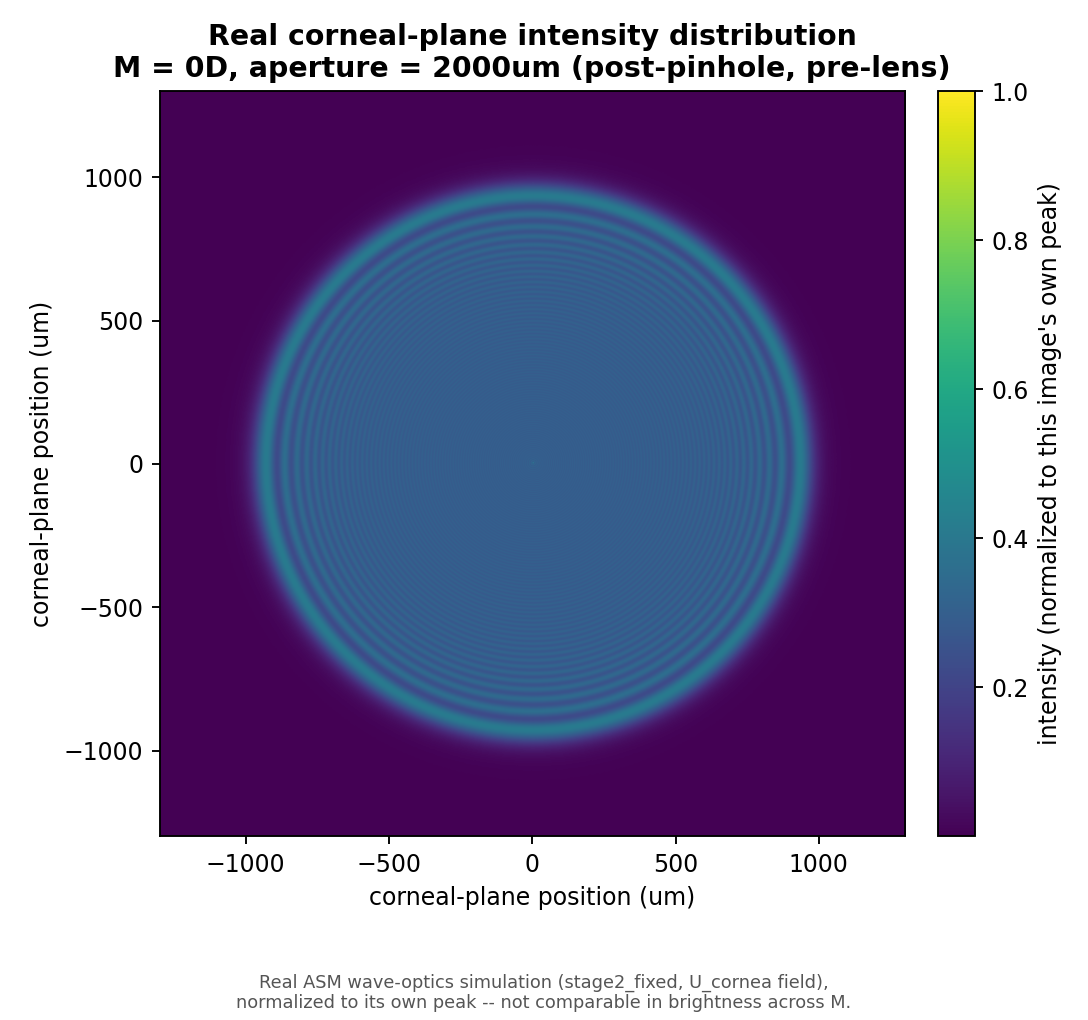
\includegraphics[width=\textwidth]{figures/corneal_illumination_M0.png}
\end{minipage}
\hfill
\begin{minipage}{0.48\textwidth}
\centering
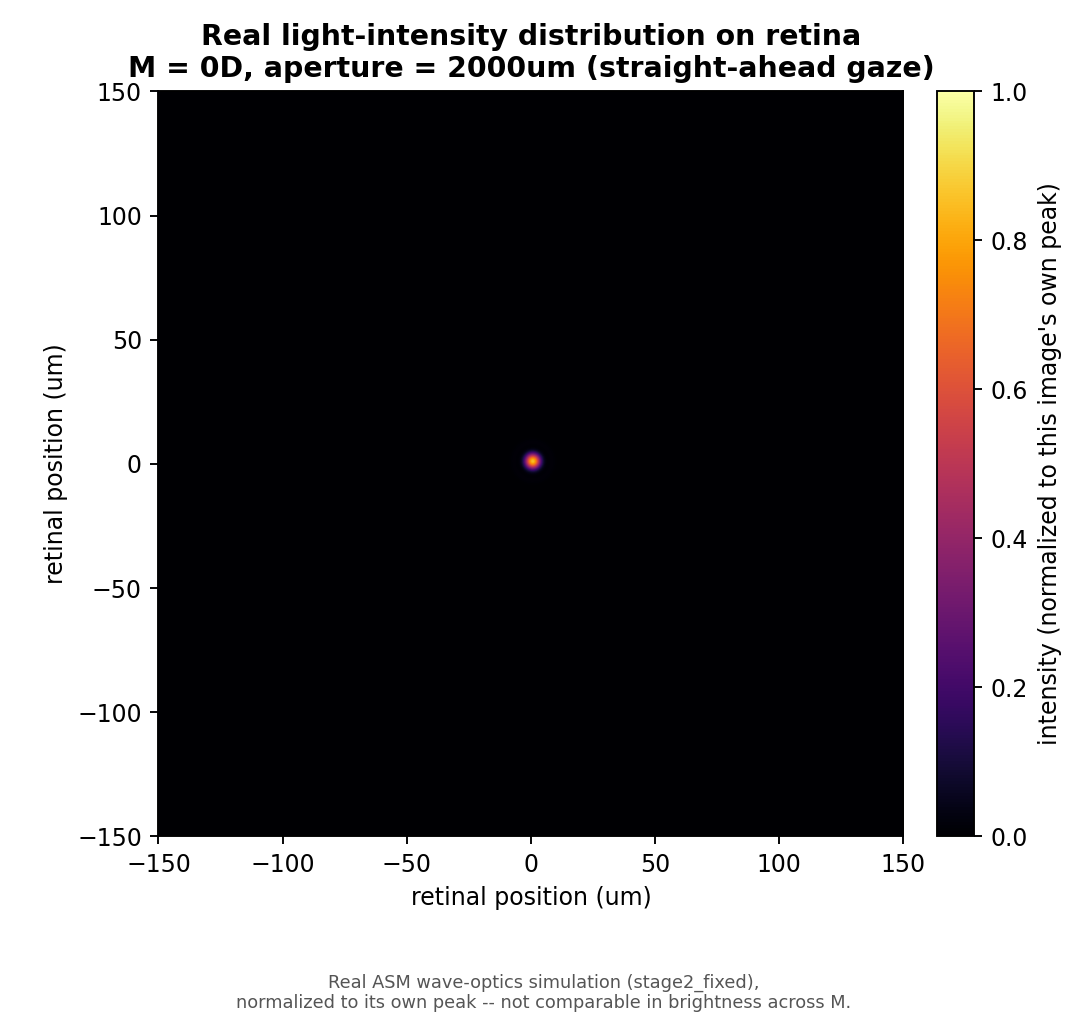
\includegraphics[width=\textwidth]{figures/realistic_heatmap_M0.png}
\end{minipage}

\vspace{6pt}
\begin{minipage}{0.48\textwidth}
\centering
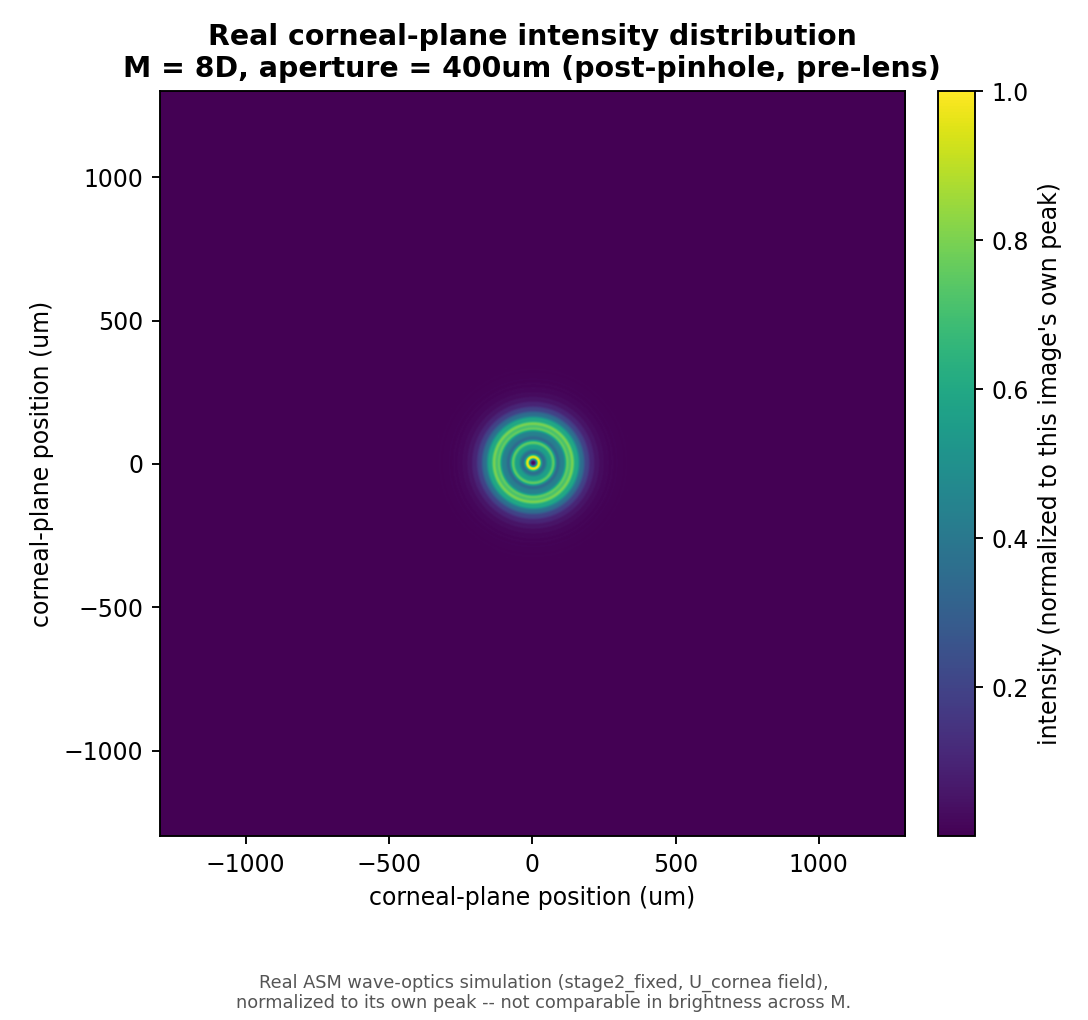
\includegraphics[width=\textwidth]{figures/corneal_illumination_M8.png}
\end{minipage}
\hfill
\begin{minipage}{0.48\textwidth}
\centering
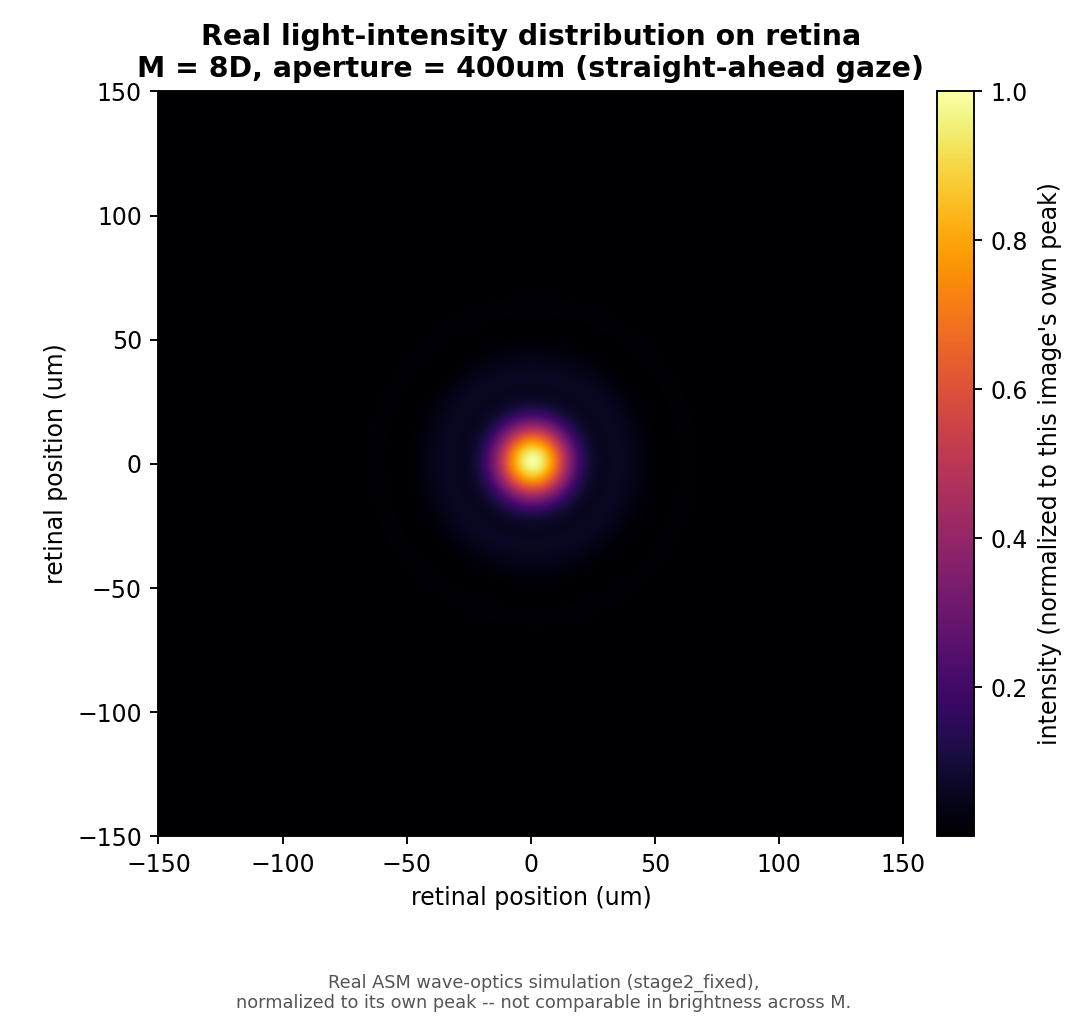
\includegraphics[width=\textwidth]{figures/realistic_heatmap_M8.png}
\end{minipage}
\caption{The pipeline chain made concrete: real $|U|^2$ intensity at the corneal
plane (left column, step~1 of the chain above, post-pinhole/pre-lens) versus the
real retinal intensity after the full lens-phase and myopic-axial-distance
propagation (right column, step~5). Top row $M=0$D, $a_{\mathrm{hole}}=2000\,\mu$m;
bottom row $M=8$D, $a_{\mathrm{hole}}=400\,\mu$m -- the two extremes of the real
per-$M$ aperture map (\texttt{array\_data/evaluation\_results/}
\texttt{PRIMARY\_WINNER\_PER\_M.csv}, mtime 2026-09-13 14:10). The corneal-plane
panels show genuine near-field Fresnel ringing at the aperture edge -- the field
has propagated only $d_{\mathrm{gap}}=12$\,mm and still closely resembles the
aperture's own geometric shape; the retinal panels show the same energy after the
myopic axial propagation, now dominated by defocus blur rather than the aperture's
edge structure. Both column pairs generated by the same
\texttt{run\_pipeline\_point()} call (one call yields both fields; no extra
propagation was run to make this comparison) --
\texttt{figure\_scripts/build\_corneal\_illumination.py} (this paper, new) and
\texttt{Array\_Design/array\_geometry\_lab/retinal\_light\_distribution\_simulation/}
\texttt{realistic\_heatmaps/build\_realistic\_heatmaps.py} (mtime of its outputs:
2026-09-28 11:15--11:16). Each panel normalized to its own peak -- absolute
brightness is not comparable across panels without a source-power calibration this
project has not made (Section~\ref{sec:limitations-optics}).}
\label{fig:cornea-vs-retina}
\end{figure}

\subsection{The effective-wavelength correction}
\label{sec:wavelength-correction}
The lens phase screen and the retina-propagation step must use the \emph{same}
effective wavelength -- $\lambda_{\mathrm{eff}}=\lambda/n'$ when
\texttt{refractive\_index\_correction=True} (this project's default), else the raw
vacuum wavelength $\lambda$. This effective wavelength is resolved \emph{once}, in
\texttt{run\_pipeline\_point}, and threaded through both the lens-phase and
retina-propagation calls -- a design choice made specifically because an earlier
version of this project's code did not do this (Section~\ref{sec:bug-fft}, the
single-FFT defocus-plane bug and its root cause both trace to exactly this
wavelength-consistency issue).

\section{Fresnel number: which diffraction regime a given stage is in}
\label{sec:fresnel-number}
\begin{equation}
N_F = \frac{R_{\mathrm{hole}}^2}{\lambda z}
\end{equation}
$N_F \ll 1$ corresponds to the far field (a clean Airy pattern); $N_F \sim 1$--$10$ is
the Fresnel transition regime (several comparably-bright diffraction rings); $N_F \gg
10$ is near-geometric (a sharp-edged projected patch, diffraction a small correction).
This project's own sweeps span Fresnel numbers well under 1 to over 20 across the
full aperture$\times$myopia grid (source:
\texttt{Array\_Design/array\_geometry\_lab/Physics\_Guide/MASTER\_HANDBOOK.tex} Chapter 6)
-- i.e.\ the mask-to-cornea and lens-to-retina propagation stages routinely sit in
\emph{different} regimes from each other within a single evaluated point, which is the
direct justification for using the regime-agnostic exact method (Equation~\ref{eq:asm})
rather than a regime-specific closed form for either stage.

\section{Numerical implementation: grid, band-limiting, and energy accounting}
\label{sec:numerics}
The ASM integral is evaluated on a finite square grid of $N\times N$ samples spanning a
physical window $L$ (so pixel pitch $dx=L/N$), via FFT. Two numerical issues require
explicit handling, both already present in the implementation and both logged, not
silently corrected:

\textbf{Band-limiting.} A finite grid cannot represent spatial frequencies beyond its
own Nyquist limit; a hard-edged pinhole mask has high-frequency content that, left
unfiltered, aliases into spurious fine structure that is numerically indistinguishable
from genuine diffraction structure. The Matsushima band limit \citep{matsushima2009} suppresses spectral
content beyond the angle at which this aliasing would occur; every run logs the
suppressed energy fraction explicitly, rather than treating it as an unaccounted loss.

\begin{keybox}{Why the energy-conservation check itself needed correcting}
Since the propagation kernel $H$ in Equation~\ref{eq:asm} has unit modulus on every
retained (propagating) spectral component and is exactly zero on every suppressed
(evanescent or band-limited) one, the apparent energy loss after propagation is
\emph{identically} the band-limit-suppressed spectral fraction:
$\varepsilon_{\mathrm{energy}} \equiv f_{\mathrm{suppressed}}$ -- confirmed against this
project's own sweep data at correlation $1.000000$ (source: \texttt{MASTER\_HANDBOOK.tex}
Chapter 6, ``Numerical band-limiting''). An energy-conservation test written against a
flat tolerance (``energy in must equal energy out to within $\epsilon$'') would
therefore fail on \emph{every single row} from this intentional, already-accounted-for
suppression alone, never distinguishing it from a genuine bug. The corrected test
instead checks the \emph{residual}
$\varepsilon_{\mathrm{energy}} - f_{\mathrm{suppressed}}$, which is near zero when the
implementation is correct and would flag a real discrepancy if one existed -- restoring
the check's actual diagnostic power.
\end{keybox}

\section{Grid-resolution artifact and the grid$\_N$ fix}
\label{sec:gridN}
A specific, separate numerical defect was found and fixed during this project's own
development, independent of the physics above: the ASM propagation grid resolution
$N_{\mathrm{grid}}$ defaults to $2048$ in
\texttt{stage4\_human\_vision/pipeline.py}'s \texttt{run\_stage4\_point} function
(verified: line \texttt{grid\_N=2048} in the function signature, current file). At this
resolution, computed blur radii for \emph{large} apertures ($\gtrsim1500$--$2000\,\mu$m)
come out approximately \textbf{2$\times$ too large} compared to the converged value at
$N_{\mathrm{grid}}=4096$ -- a genuine numerical under-resolution artifact, not a
physical effect. \texttt{new\_sweeps/run\_blur\_sweep.py} was corrected to pass
$N_{\mathrm{grid}}=4096$ explicitly on 2026-08-16; the acuity-model sweep script,
\texttt{new\_sweeps/run\_acuity\_sweep.py}, called the same underlying function but was
\emph{not} updated to match until 2026-09-12/13, leaving every acuity-model number
computed from that script stale for nearly a month. This specific staleness episode,
its full blast-radius accounting, and its remediation are documented as a worked case
study in Section~\ref{sec:bug-gridN}.

\section{Validation of the ASM engine}
\label{sec:asm-validation}
At the closed-form-tractable limit ($d_{\mathrm{gap}}\to0$, $M=0$), the pipeline output
was checked directly against the exact Fraunhofer diffraction result for a circular
aperture:
\begin{equation}
I(r) = I_0\left(\frac{2J_1(x)}{x}\right)^2, \qquad x = \frac{\pi a r}{\lambda v_r},
\qquad
EE(x) = 1 - J_0^2(x) - J_1^2(x)
\end{equation}
Agreement is within 2\% on the 50\%- and 90\%-encircled-energy radii. The 80\%-radius
check needs 8\% tolerance: the first Airy-pattern null sits at $x=3.8317$, where
$EE\approx0.838$ -- almost exactly the 80\% level, on a flat part of the encircled-energy
curve where a small energy error maps to a disproportionately large radius error.
Repeating the check at grid sizes from 1024 through 8192 never brought this residual
below 2.3--4.6\%, confirming it is genuine ill-conditioning of that specific percentile
at that specific aperture regime, not an under-resolved grid (source:
\texttt{MASTER\_HANDBOOK.tex} Chapter 6, ``Validation against the closed form'').

Separately, the on-axis intensity was checked against the closed-form Fresnel-zone
oscillation $I(0,z)=4I_0\sin^2(\pi N_F/2)$ and matched at correlation $0.997$ -- direct
confirmation that the non-monotonic Strehl-ratio behaviour this project's sweeps show
(multiple local maxima as aperture is swept at fixed $M$) is real Fresnel-zone
interference, not numerical noise, and is one of the reasons the RSS model
(Section~\ref{sec:rss}), which is smooth and monotonic by construction, cannot
represent this project's own actual blur behaviour.

\section{Blur metrics and where each one breaks}
\label{sec:blur-metrics}
\begin{center}
\begin{tabular}{p{2.6cm}p{4.8cm}p{6.0cm}}
\toprule
Metric & Measures & Failure mode \\
\midrule
$r_{EE}(50\%)$ & Radius enclosing half the retinal energy & Stable and monotonic in
aperture, but overestimates clinical acuity loss by roughly $7\times$ against measured
clinical data (Chapter~\ref{ch:model-comparison}) \\
FWHM & Width of the central diffraction/blur core only & Tracks clinical acuity loss
more closely ($\sim1.6\times$) but is \emph{discontinuous} in the design variable: a
jump from $4.7\,\mu$m to $154.7\,\mu$m was observed between two apertures only
$250\,\mu$m apart at $M=4$D, from ring-hopping between local intensity maxima \\
Strehl ratio & Peak intensity relative to the diffraction limit & Genuinely
multi-peaked (6--7 local maxima across the aperture sweep at fixed $M$), confirmed
\emph{worse} (more, not fewer, peaks resolved), not numerically better, at $10\times$
finer grid sampling -- i.e.\ this is real physics (matched to the Fresnel-zone
closed form above), not numerical noise to be smoothed away \\
\bottomrule
\end{tabular}
\end{center}

\begin{keybox}{Why $r_{EE}(50\%)$ is used as the project's standard optimization metric anyway}
Per individual aperture, FWHM is unusable as an optimization target because it is
discontinuous in the very variable being optimized. Across a coarse sweep its
\emph{trend} tracks clinical reality more closely than $r_{EE}(50\%)$, which is smooth
and numerically well-behaved but systematically pessimistic by roughly $7\times$. This
project reports $r_{EE}(50\%)$ as its blur-optimization metric throughout and states its
known bias explicitly, rather than optimizing against a metric that is discontinuous in
the design variable it is meant to optimize.
\end{keybox}

\section{Deprecated formulas}
\label{sec:deprecated}
\begin{center}
\begin{tabular}{p{5.4cm}p{7.4cm}}
\toprule
Formula & Status and measured error \\
\midrule
$r_{\mathrm{geo}} = \dfrac{a_{\mathrm{hole}}}{2}\dfrac{|v_r-v_f|}{v_f}$ & Deprecated.
Superseded by the direct ASM chain (Section~\ref{sec:asm}), which produces this effect
automatically without a separate geometric-blur term. \\
$r_{\mathrm{tot}}=\sqrt{r_{\mathrm{geo}}^2+r_{\mathrm{diff}}^2}$ (RSS,
Section~\ref{sec:rss}) & Deprecated. 64.8\% mean, 192.8\% maximum divergence from the
exact result. \\
$a_{\mathrm{eff}}\approx\sqrt{a_{\mathrm{hole}}^2+(2.44\lambda d_{\mathrm{gap}}/a_{\mathrm{hole}})^2}$
& Deprecated. Smooth and monotonic by construction; cannot represent the genuine
Fresnel-zone oscillation confirmed in Section~\ref{sec:asm-validation}. \\
\bottomrule
\end{tabular}
\end{center}

\section{Array optics reuse single-aperture optics unmodified}
\label{sec:array-vs-single}
Every hole in a fabricated array has optics \emph{identical} to a standalone single
aperture of the same diameter $a_{\mathrm{hole}}$ at the same myopia power $M$: the
array geometry changes only whether zero, one, or multiple holes' images
simultaneously reach the retina (blinding, clean imaging, or ghosting -- Chapter
\ref{ch:array-theory}), never the per-hole blur itself. This is why every array
evaluation result in this paper (Chapters~\ref{ch:model-a}--\ref{ch:model-b}) looks up
its predicted acuity directly from the single-aperture sweep at the array's own chosen
aperture, rather than re-deriving acuity per array family -- a claim independently
confirmed in this paper's own analysis (Section~\ref{sec:model-comparison-table}): all
six array evaluation models tested produce numerically identical predicted LogMAR per
myopia power, differing only in which \emph{geometry} carries that identical optical
aperture.
